\chapter{Introduction}\label{ch:introduction}

% Stars are the fundamental building blocks of the universe. Their evolution directly affects the evolution of their host galaxies, and in turn that of the universe.

Massive stars have initial masses larger than eight times the mass of our sun (M$_i \gtrsim 8$\,\Msun{}) and are fundamental cosmic engines. Through their strong stellar winds, intense radiation and powerful explosions, they dominate the transport of energy and momentum into the interstellar medium \citep[][]{mac_low_distribution_2005}. The final explosions of massive stars are so bright that they can be seen throughout the universe and allow the study of its properties across cosmic times \citep{tanvir_-ray_2009}. The first generation of massive stars are thought to have played a pivotal role in the assembly of the first galaxies \citep{bromm_first_2004,robertson_early_2010}. They are potential progenitors of core-collapse supernovae (SN) and gamma-ray bursts \citep{woosley_supernova_2006}, the remnants of which are neutron stars (NS) and black holes (BHs). In binary systems, these compact objects can undergo coalescence to produce intense bursts of gravitational waves.

Despite their importance in a variety of astrophysical phenomena, there remain major uncertainties in our understanding of massive stellar evolution. Processes such as internal mixing, rotation, magnetic fields and multiplicity are few of the numerous parameters that strongly affect the mass, and hence evolution, of a star. In the past decades, observational surveys have shown that multiplicity is the rule, and not the exception, among massive OB-type stars \citep{mason_iccd_1998,mason_high_2009,sana_binary_2012,sana_vlt-flames_2013,sana_southern_2014,kobulnicky_toward_2014,barba_own_2014,dunstall_vlt-flames_2015,maiz_apellaniz_galactic_2016,maiz_apellaniz_monos_2019,almeida_tarantula_2017,banyard_observed_2022,villasenor_b-type_2021}. Most of the stars in these systems will interact with their companions \citep{fryer_constraints_2007,sana_binary_2012,sana_vlt-flames_2013,dunstall_vlt-flames_2015}, thereby fundamentally impacting the evolution of most of these systems \citep{paczynski_evolution_1967,pols_case_1994,1998Vanbeveren_popsynth,2014deMink_mergers}. This thesis mainly addresses the aspect of multiplicity in a subset of massive stars, called Wolf-Rayet (WR) stars, from an observational standpoint. This Chapter provides a brief introduction on stellar evolution, summarises the characteristics of WR stars, dives into the Galactic population of WR stars and provides the motivation for this thesis.

% \section{Stellar evolution in a nutshell}

% The birth of a star starts with a cold, dense molecular cloud. When a perturbation is applied to this cloud, say from a nearby supernova, parts of this cloud could undergo compression and gravitational collapse. This cloud could then undergo fragmentation, forming smaller clumps of dust that are the progenitors of single and multiple stars. The surrounding matter continues to fall onto each of these clumps, forming circumstellar disks through which accretion occurs. Even after the fragmentation process ends, the clumps of material continue to contract. This results in an increase in the central density, causing the central temperature to rise. As the material heats up, it radiates the energy away in the form of infrared radiation. The protostar continues to heat up and contract, dissociating molecular hydrogen into its atomic form. The star contracts and heats up until the core reaches a temperature of ${\sim}10^6\,$K, which is when it can start burning hydrogen. When hydrogen burning becomes the dominant energy production in the star (as compared to contraction), the star is said to be entering its main-sequence phase. The star spends most of its lifetime on the main sequence, until all the hydrogen in its core is converted to helium through nuclear fusion. It will then go through a cycle of contraction and fusion of helium, carbon, etc. in its core.

% \begin{figure}
%     \centering
%     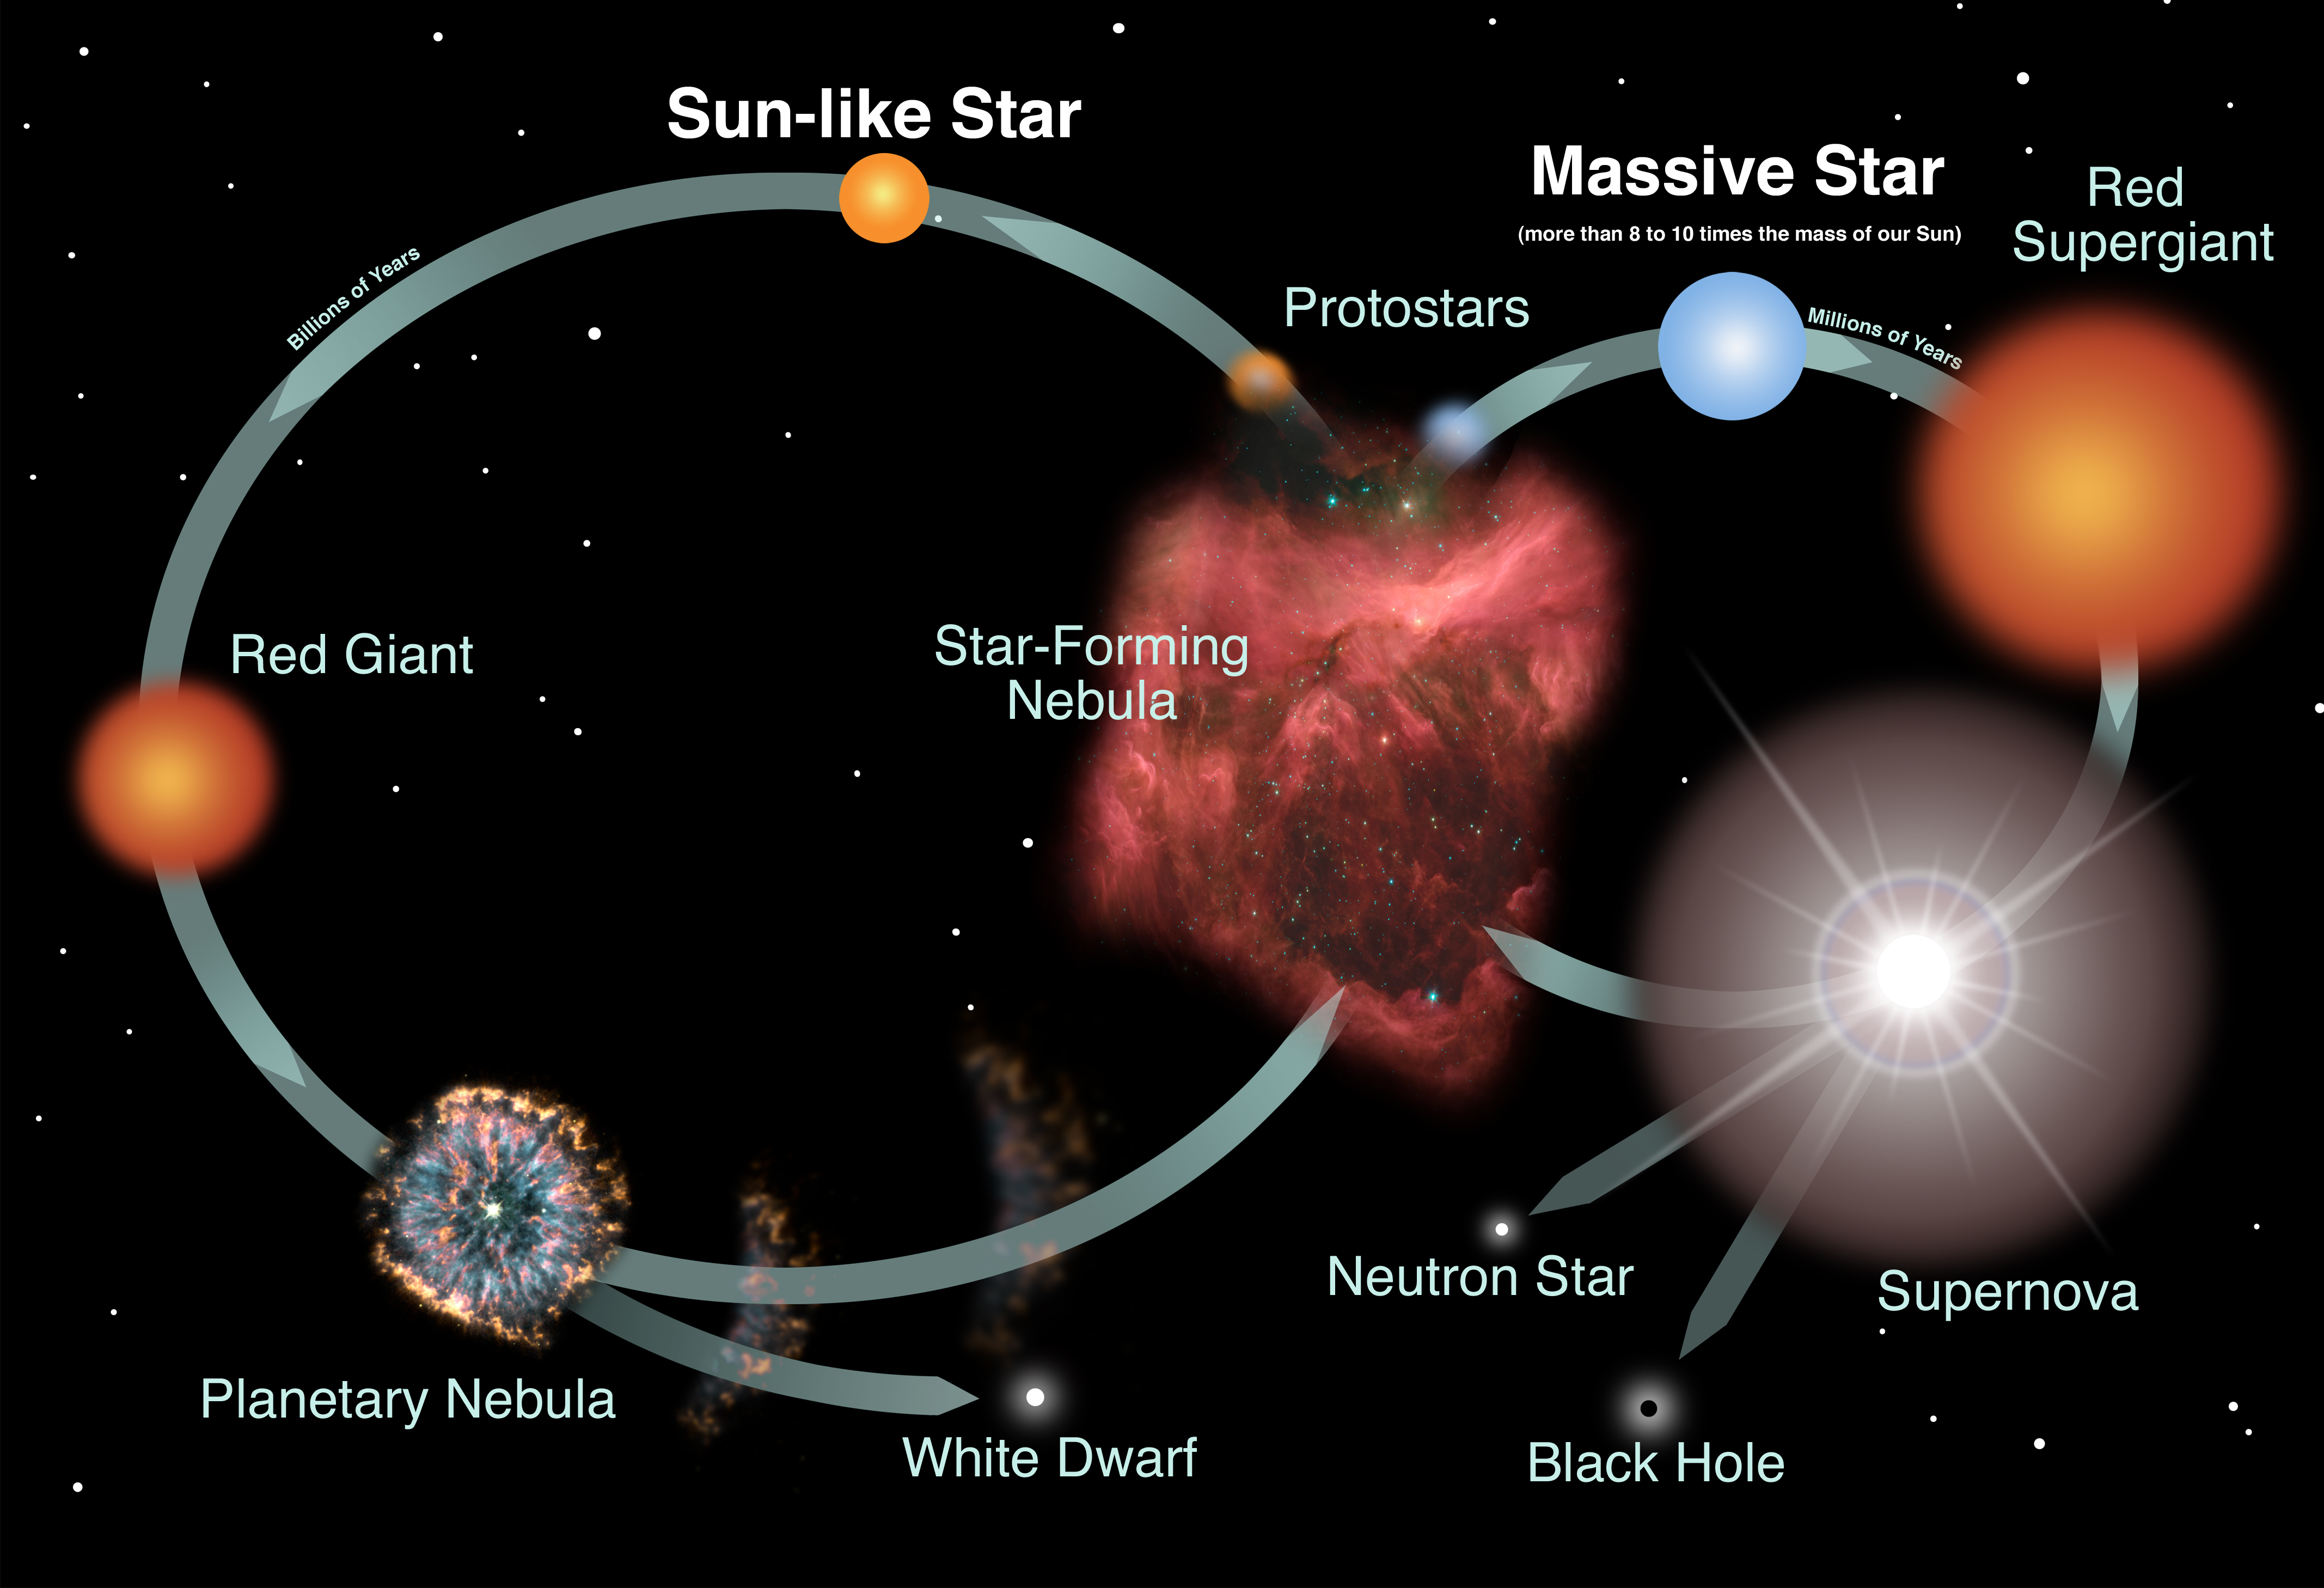
\includegraphics[width=0.9\textwidth]{Chapters/introduction/image/stars_lifecycle_full.jpeg}
%     \caption{Life cycle of a star. Left: evolution of a low-mass star like the sun. Right: evolution of a massive star ($M_i \gtrsim8\,$\Msun{}). \textbf{Credit:} NASA.}
%     \label{fig:lifecycle}
% \end{figure}

% The evolution from here on is governed by the initial mass of the star (Fig. \ref{fig:lifecycle}). Low mass stars $M_i \lesssim 8\,$\Msun{} will end up with a degenerate carbon/oxygen core where no further nuclear fusion can occur. These stars will end their lives as a carbon/oxygen white dwarf, shedding their outer envelope to form a planetary nebula. Stars with initial masses between 8 and 25\,\Msun{} will evolve past the main sequence and enter the red-supergiant (RSG) phase before ending their lives as Type II (hydrogen-rich) SN.

% Stars with initial masses more than 25\,\Msun{} are thought to avoid the cooler supergiant phase, instead experiencing strong mass-loss through stellar winds or through episodic eruptive events in the luminous blue variable (LBV) phase. After the LBV/RSG phase, these stars may appear as WR stars. This phase is short-lived (${\sim}10$\% of the stellar lifetime) after which they end their lives either as Type Ib/c supernovae or through direct collapse, leaving behind NS or BHs \citep{heger_how_2003}.

%  On the other hand, massive stars with $M_i \gtrsim 8$\,\Msun{} will fuse carbon, oxygen and so on in their cores until they end up with a degenerate iron core. In the post main-sequence phase of their evolution, m

\section{Wolf-Rayet stars}\label{sect:wr_intro}

\textit{The content of this section is mainly based on \citet{crowther_physical_2007} and \citet{langer_presupernova_2012}.}

A small subset of massive stars appear as WR stars. The class is named after French astronomers Charles Wolf and Georges Rayet, who in 1867 observed and identified three stars in the constellation Cygnus whose spectra showed spectacularly broad and strong emission lines, particularly of He\,{\sc ii} $\lambda 4686$ and H$\beta$. In the context of stellar evolution, WR stars are candidate progenitors of core-collapse SN and BHs, making their study quintessential in understanding the initial properties of such phenomena.

\subsection{Observational characteristics}\label{sect:wr_obs_char}

WR stars comprise a spectral class of stars with emission-line dominated spectra. They appear in multiple ``flavours'' based on the chemical composition of their atmospheres: nitrogen-rich (WN), carbon-rich (WC), and the rare oxygen-rich (WO) sequences (Fig. \ref{fig:spectypes}). Based on the strengths and ratios of various emission lines, WN and WC stars are also sub-classified as early (WNE: WN2-WN5, WCE: WC4-6) or late (WNL: WN6-WN9, WCL: WC7-9) following the convention from \citet{smith_revised_1968}. The spectral types of WN stars can be suffixed by `h' or `o' depending on the presence or absence of hydrogen in the spectra.

\begin{figure}
    \centering
    % 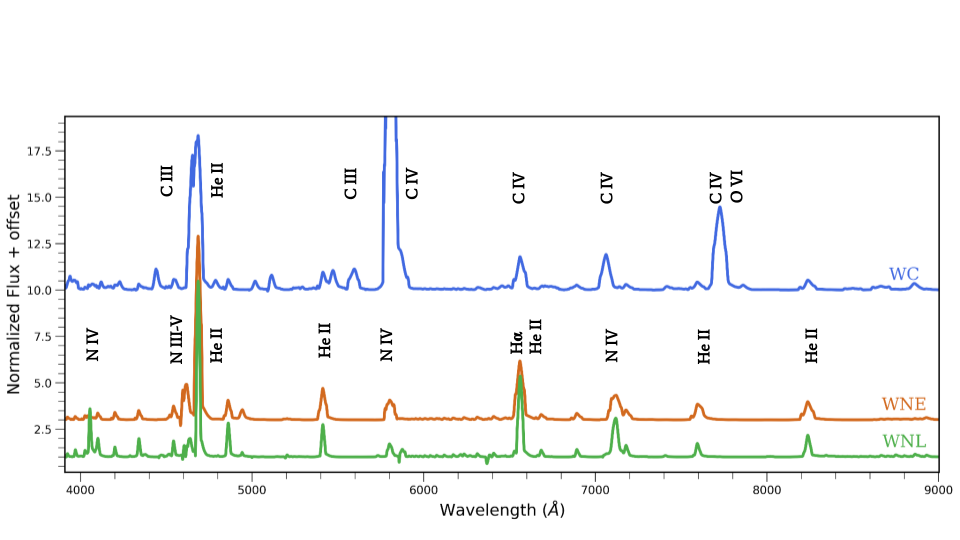
\includegraphics[width=\textwidth]{Chapters/introduction/image/Spectypes.png}
    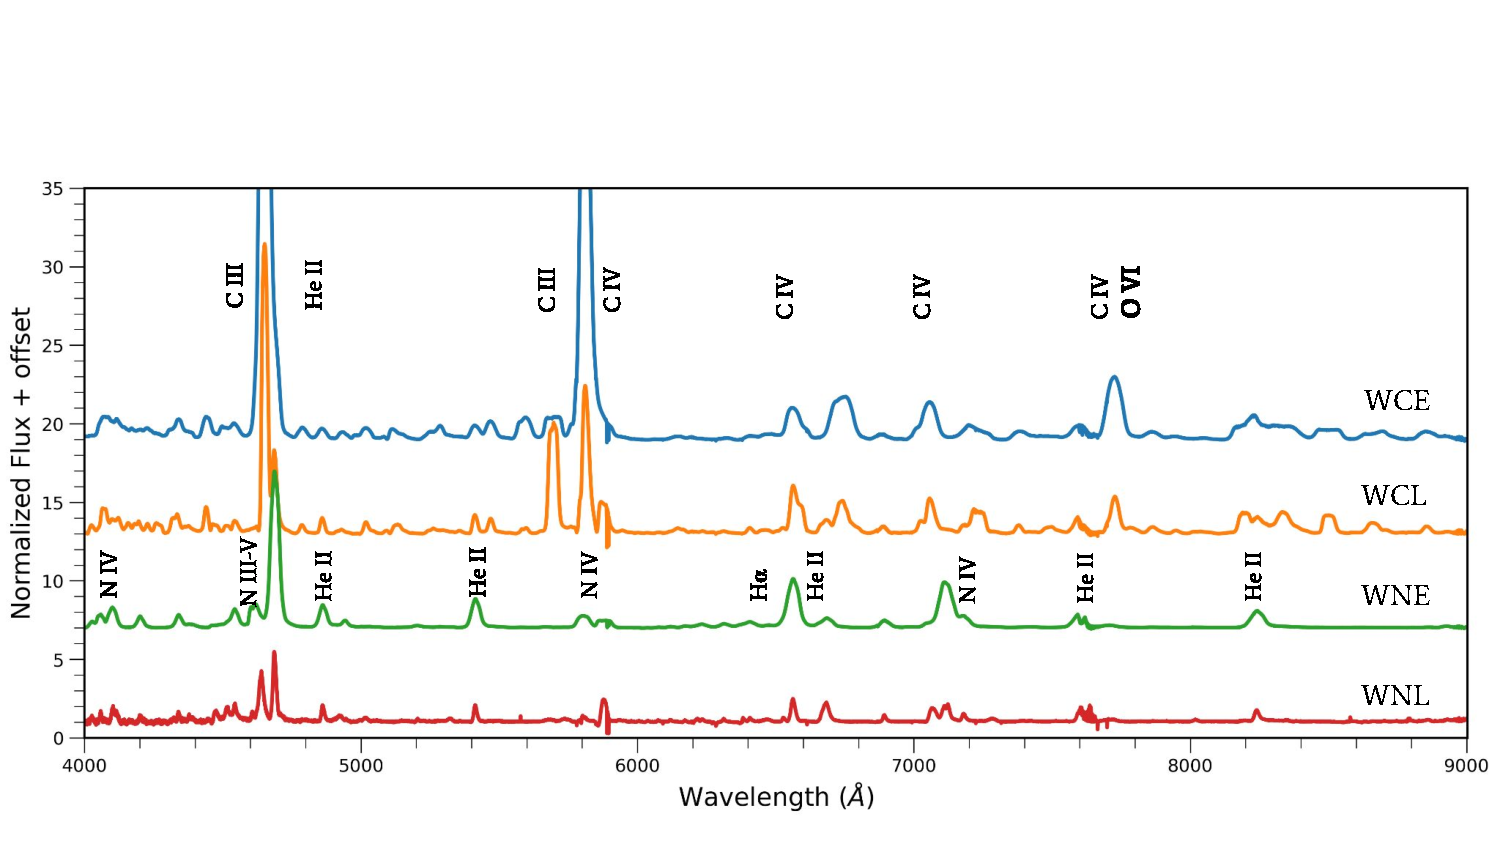
\includegraphics[width=\textwidth]{chapters/introduction/image/Obs_SpT.pdf}
    \caption{HERMES spectra of WR 111 (WCE), WR 135 (WCL), WR 6 (WNE) and WR 120 (WNL) demonstrating the different spectral features of the various WR sub-types in the Galaxy. The spectra are rebinned for clarity and plotted with an offset, with various spectral lines indicated in black.}
    % \caption{HERMES spectra of WNE (WR 6; WN4b), WNL (WR 120; WN7o), WCE (WR 111; WC5) and WCL (WR 135; WC8) sub-types in the Galaxy. The spectra are rebinned for clarity and plotted with an offset, with various spectral lines indicated in black.}
    \label{fig:spectypes}
\end{figure}

The optical emission-line spectra of WR stars are primarily constituted by recombination lines. The strength of these lines depend on the number of electrons and ions in the outflowing wind, and hence scale with the square of the density. This is why the spectral appearance of a WR and O star are drastically different, despite the wind density changing by only a factor of 10 or so. The high density in the wind also results in a high optical depth, such that the photosphere (hydrostatic layers) is hidden from sight. Therefore, the spectra of WR stars are formed in the geometrically-extended, fast-moving stellar wind. As a result, it is challenging to obtain information about the stellar parameters through spectroscopic analysis, as this requires an in-depth understanding of the structure of the wind.

WR stars are notorious for their line-profile variability \citep{lepine_wind_1996,lepine_wind_2000,st-louis_systematic_2009,chene_systematic_2011,chene_clumping_2020}. This is usually attributed to inhomogeneities in the wind, which results in the spectral lines of WR stars changing their appearance over time. Periodic change in the equivalent widths and the full-width half maximum of line profiles has even led to speculations of binary companions \citep[e.g. WR 1][]{morel_investigation_1999}. In the recent years, it has been shown that certain WR stars harbour large-scale structures that could cause such periodicity \citep[e.g.][]{st-louis_measuring_2008,aldoretta_extensive_2016,st-louis_polarization_2018}. The photometry of WR stars also shows quasi-periodic variability on short timescales \citep[e.g.][]{moffat_photometric_1986,balona_intensive_1989,st-louis_brite_2020}, which have been attributed to non-radial pulsations, co-rotating interaction regions (CIRs) or binary companions.

WR stars are usually found in isolated regions, although a fair fraction of them in the Galaxy are found in young clusters \citep{rosslowe_spatial_2015}. A small fraction of WR stars also have nebulae surrounding them, showing a variety of morphological features \citep{toala_wise_2015}. These nebulae are often associated with young WR stars, particularly WN sub-types, although some have been found around WC stars. The nebulae are a result of strong, UV radiation from the WR star interacting with and photo-ionizing the material ejected in a past RSG/LBV phase.

Since the WR phenomenon is defined by observational, spectroscopic characteristics, multiple objects come under the umbrella term. There are three main types of stars that are classified as WR stars:

\begin{itemize}
    \item \textbf{Main-sequence WR stars:} stars with initial masses ${\sim}80\,$\Msun{} and higher have winds so strong that they can exhibit a WR-like appearance while burning hydrogen in their cores. They show lines of hydrogen in their spectra and are called WNh stars.
    \item \textbf{Classical WR stars:} these are hydrogen-depleted, helium-rich stars that are thought to be the descendants of WNh and main-sequence O stars with initial masses from 25\,\Msun{} and above. Having evolved off the main sequence in the HR diagram, these stars are no longer burning hydrogen in their cores. They are called cWR stars, and are potential candidates as progenitors of type-Ib/c supernovae.
    \item \textbf{Central stars of planetary nebulae:} as relatively massive post-ABG stars evolve into planetary nebulae, the inner core that is exposed is hot enough to drive strong winds, appearing as WR stars. These are often referred to as [WR] stars.
\end{itemize}

In this work, we refrain from discussing [WR] stars which stem from lower-mass ($M_i < 8\,$\Msun{}) objects and focus on classical- and main-sequence WR stars.

\subsection{Stellar winds}

The high temperatures and luminosities of massive stars imply that most of their radiation is in the UV. Given the plethora of spectral lines present in the UV domain (mainly of iron), this radiation induces a force strong enough to drive material away from the star. This stream of outflowing material is then called a radiation-driven stellar wind \citep{1970LucySolomon,1975castor}. As material is accelerated away from the star, spectral lines are Doppler-shifted due to their high velocities, and so photons with wavelengths away from the line-center can also interact with these atoms, further increasing the radiative force on the wind.

The outflows of massive stars were initially thought to be homogeneous and smooth \citep{1988deJager,1990Nieuwenhuijzen}. However, theoretical studies have indicated that clumping is expected in massive-star outflows \citep{1988Owocki,2005DessartOwocki,2013SundqvistOwocki,2018Sundqvist,2019A&A...631A.172D}. Similar to the stellar outflows of all massive stars, the winds of WR stars are also clumpy \citep{1991Hillier_clumping_escattering,1998Hamann_clumping,puls_bright_2006,fullerton_discordance_2006}.

There are a number of unanswered questions related to the atmosphere models of WR stars. First, spectroscopic observations of WR stars find WR radii much larger than those predicted by theory \citep{2007Crowther,hamann_galactic_2019,sander_galactic_2019}. This is called the WR core-radius problem. Secondly, the structure of WR winds are still a point of research, as the launching mechanisms in one-dimensional optically thick winds fail to sustain a stellar wind that can escape the stellar potential \citep[e.g.][]{2016Ro_WR_winds,2017Sander_WR_winds}. \citet{2021Poniatowski} showed that WR winds can be launched with a hybrid-opacity model, and that the inner regions of WR winds are dynamically inflated. This also provides a potential solution to the WR core-radius problem. Three-dimensional radiation-hydrodynamic simulations by \citet{2022Moens} have shown that, for sufficiently-high luminosities, the winds can be launches from the deep sub-surface regions. Moreover, their simulations also predict structure in the winds of WR stars. Comparing observational time-series data of spectra \citep[e.g.][]{lepine_wind_2000} with synthetic predictions to constrain wind parameters is something that is now feasible.

\subsection{Formation and evolution of WR stars}

\textit{The content of this section is mainly from \citet{crowther_physical_2007} and \citet{shenar_why_2020}.}

\begin{figure}
    \centering
    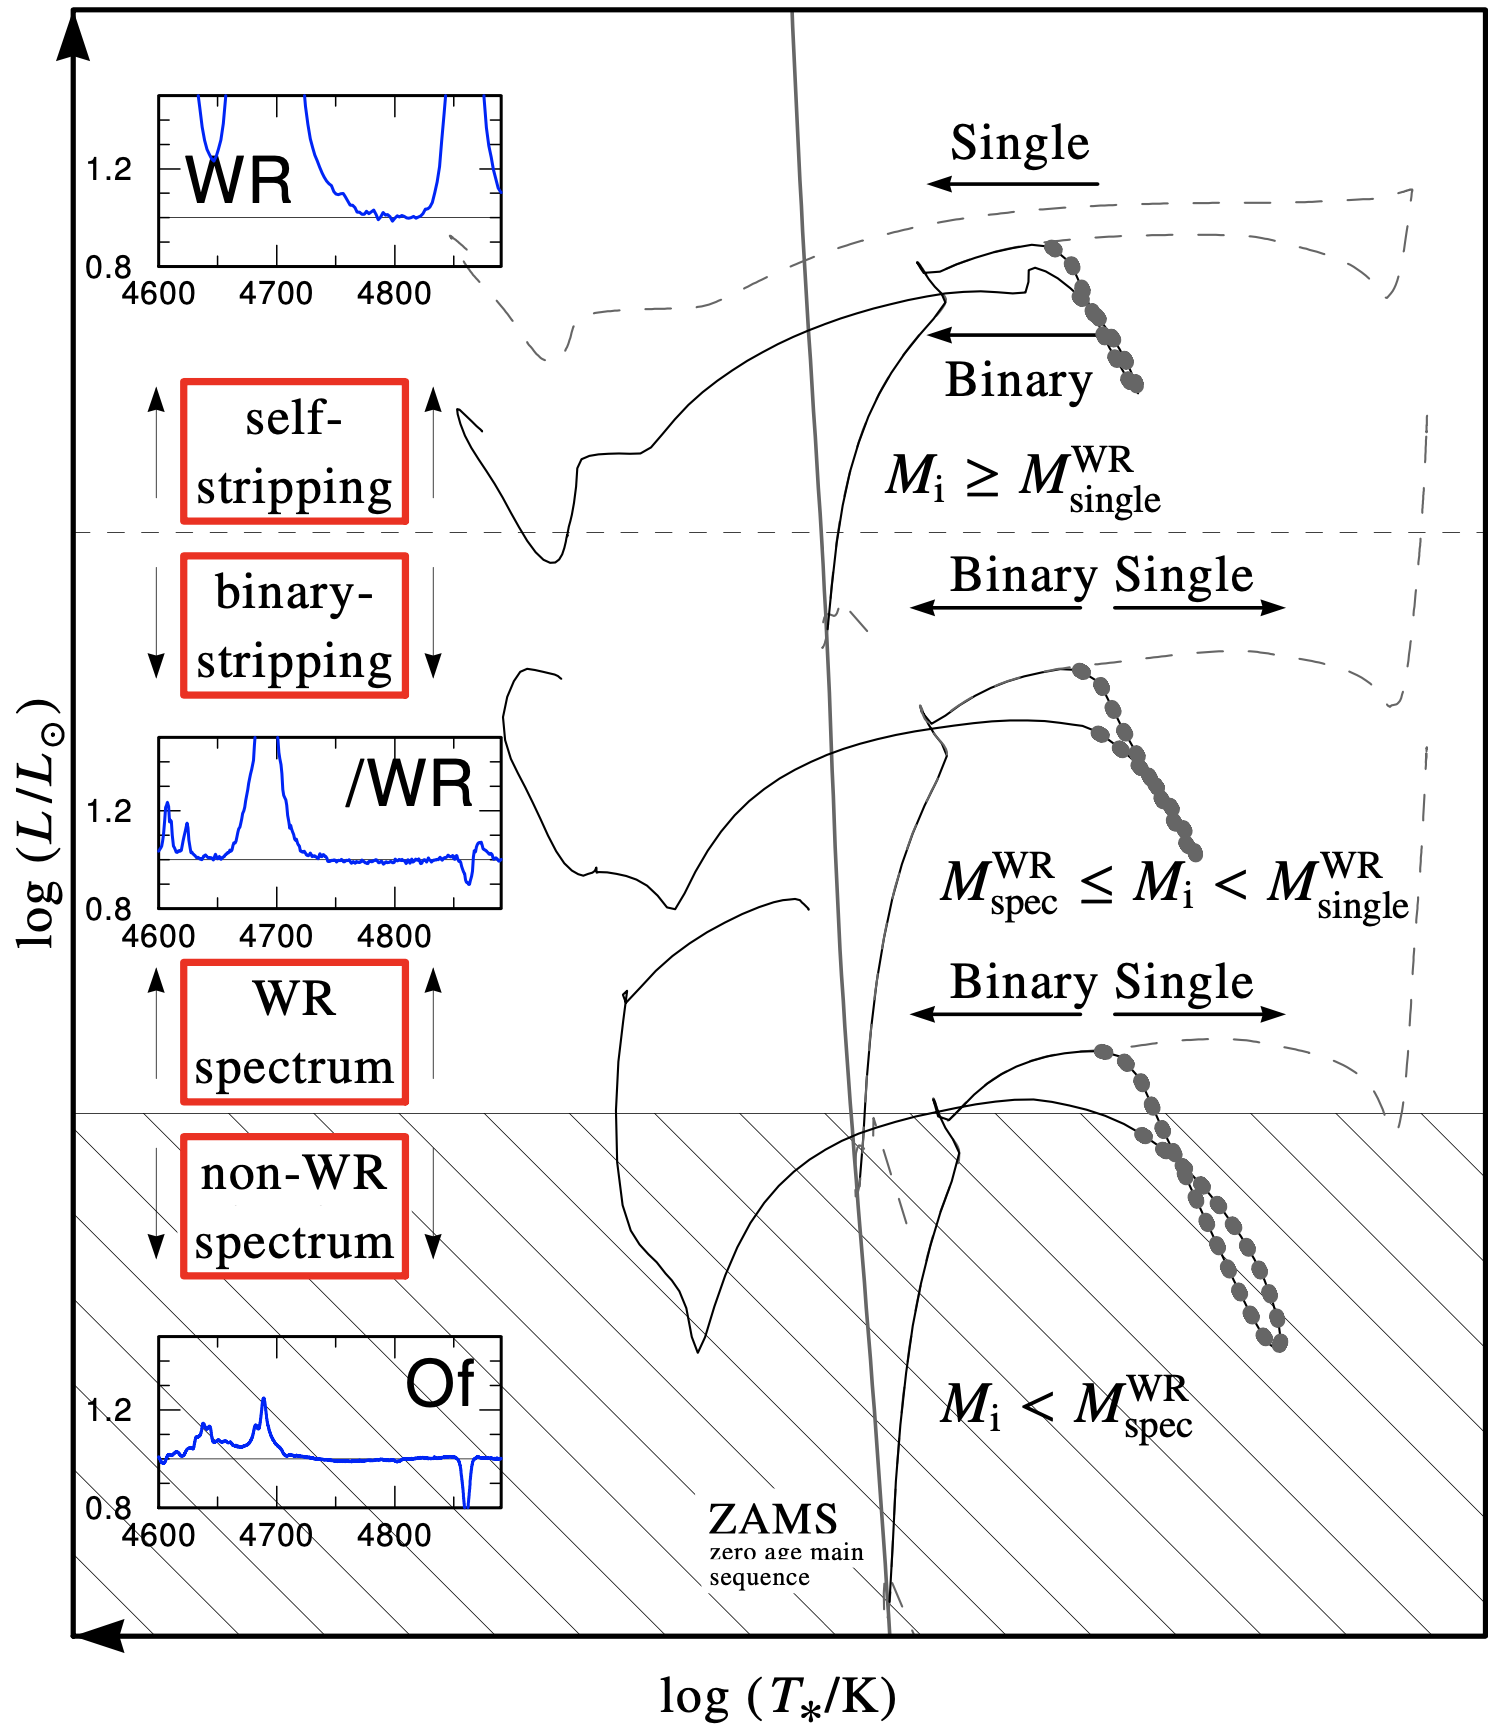
\includegraphics[width=0.6\textwidth]{chapters/introduction/image/FormationChannels.png}
    \caption{An illustration of the different formation channels through which WR stars can be formed. $M^{\textrm{WR}}_{\textrm{single}}$ is the minimum initial mass for a star to be able to strip itself via stellar winds. $M^{\textrm{WR}}_{\textrm{spec}}$ is the minimum initial mass required for a star to appear as a WR star \textit{after} being stripped. Figure adopted from \citet{shenar_why_2020} with stellar evolution models from BPASS.}
    \label{fig:formation_wr}
\end{figure}

\citet{gamow_wc_1943} first suggested that the chemical composition of the spectra of WR stars showed the products of nuclear fusion in the core of massive O-type stars. For this to be possible, an O star has to shed its hydrogen-rich envelope. An explanation was provided by \citet{paczynski_evolution_1967}, who explained that this was possible through mass-transfer in close binaries. This led to the initial claim that all WR stars were the product of binary interaction. Soon after this, Peter Conti hypothesised that a single, massive star could shed its hydrogen envelope through mass loss via its own stellar winds. As the star further evolved, first the products of hydrogen-burning (through the CNO-cycle, nitrogen) and then helium-burning (through the triple-alpha process, carbon) would be exposed. This came to be known as the ``Conti evolutionary scenario'' or simply the ``Conti scenario'' \citep{1976Conti}. This explanation become more popular as it did not require external help for an O star to evolve into a WR star. O stars can also lose mass through episodic outbursts due to instabilities \citep[e.g.][]{langer_towards_1994} or due to continuum driven instabilities \citep{smith_role_2006}.

Ever since it was shown that the majority of O stars live in close binaries that will interact over the course of their lifetime \citep{sana_binary_2012}, the debate over the dominant mechanism through which the envelope of an O star is stripped is still ongoing \citep{vanbeveren_wr_1998,foellmi_wolf-rayet_2003,shenar_wolf-rayet_2019,neugent_close_2014,shenar_why_2020}. Since the opacity required for the driving of stellar winds is dependent on metallicity, the mass-loss rates of massive stars decrease with reduced metallicity \citep{vink_mass-loss_2001,vink_metallicity_2005,hainich_wolf-rayet_2015,shenar_wolf-rayet_2019}. As a result, it was thought that envelope stripping by a companion is the major formation channel at lower metallicities \citep{maeder_new_1994,smith_mass_2014,groh_grids_2019}. For example, according to \citet{meynet_stellar_2003,meynet_stellar_2005} a star with an initial mass of 25\,\Msun{} can strip itself at solar metallicity. This value increases to ${\sim}45\,$\Msun{} for the SMC, although both of these values are highly dependent on underlying assumptions. However, \citet{shenar_why_2020} have shown that while binary stripping might occur for most stars at lower metallicities, the resulting stars will not have strong enough stellar winds to appear as WR stars (Fig. \ref{fig:formation_wr}). Hence, the role of binary interactions in forming WR stars, in our Galaxy as well as across the Cosmos, remains an unsolved problem.

\begin{figure}
    \centering
    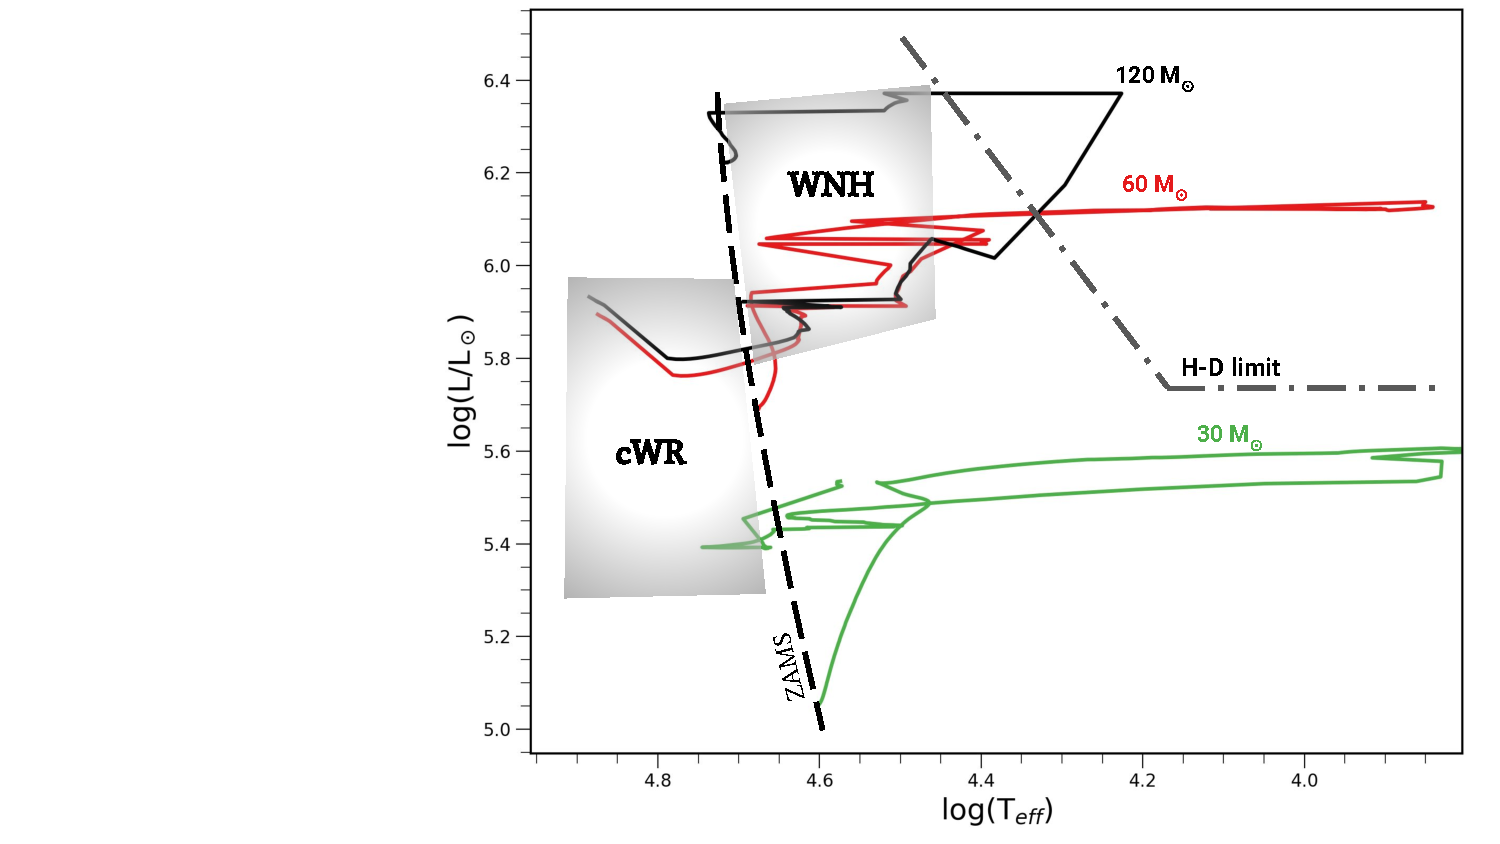
\includegraphics[width=\hsize]{chapters/introduction/image/HRD_GENEVA.pdf}
    \caption{Hertzsprung-Russel diagram showing the evolution of massive stars using tracks from the Geneva code \citep{2012Ekstrom}. Evolution tracks for initial masses of 30, 60 and 120\,\Msun{} are shown, along with the zero-age main sequence (ZAMS). The shaded grey areas are regimes where stars can appear as WNh or cWR stars.}
    \label{fig:hrd_geneva}
\end{figure}

\subsubsection{Evolution at Galacic metallicity} \label{sect:evo_galactic}

Stars with initial masses $M_i \gtrsim 25\,$\Msun{} are able to strip their envelopes via their stellar winds. They are thought to avoid the cooler supergiant phase, instead experiencing strong mass-loss through stellar winds or through episodic eruptive events in the luminous blue variable (LBV) phase. After the LBV/RSG phase, these stars may appear as WR stars (Fig. \ref{fig:hrd_geneva}). This phase is short-lived (${\sim}10$\% of the stellar lifetime) after which they end their lives either as Type Ib/c supernovae or through direct collapse, leaving behind NS or BHs \citep{heger_how_2003}.

Observational analysis of WR stars is important in understanding their mass-loss rates, radii and masses, among other parameters. For the population of single Galactic WR stars, the atmospheric-modelling work of \citet{hamann_galactic_2019} for WN stars and \citet{sander_galactic_2019} for WC stars has been significant. With distances from Gaia DR2, \citet{hamann_galactic_2019} confirmed that most WNL stars are slightly more luminous than WNE stars. \citet{sander_galactic_2019} also showed with Gaia DR2 distances that the luminosity and temperature of WC stars was, on average, similar to that of Galactic WNE stars. In their analysis, \citet{hamann_galactic_2019} also show that most, if not all, WNL stars contain hydrogen in their spectra. An updated evolutionary channel for single O stars to evolve into WR stars, based on their initial mass (modification to the Conti scenario) is given in \citet{sander_galactic_2019}. For $M_i > 80\,$\Msun{},

\centerline{O $\longrightarrow$ Of/WNH $\longleftrightarrow$ LBV  [$\longrightarrow$ WNH] $\longrightarrow$ SN IIn,}

for $35 \le M_i \le 80\,$ \Msun{},

\centerline{O $\longrightarrow$ Of/WNH $\longleftrightarrow$ LBV  $\longrightarrow$ WN $\longrightarrow$ WC $\longrightarrow$ WO $\longrightarrow$ CC,}

for $18 \le M_i \le 35\,$ \Msun{},

\centerline{O $\longrightarrow$ RSG $\longrightarrow$ WNL [$\longleftrightarrow$ LBV] $\longrightarrow$ WN $\longrightarrow$ WC $\longrightarrow$ WO $\longrightarrow$ CC,}

and for $8 \le M_i \le 18\,$ \Msun{},

\centerline{OB $\longrightarrow$ RSG [$\longrightarrow$ BSG] $\longrightarrow$ SN II}

where `CC' indicates core-collapse. The mass ranges above are not set in stone, and they are derived by comparing empirically derived luminosities to stellar evolution models. However, the specific end stages presented above are widely debated in the literature and depend on the physics included in evolutionary models \citep[e.g., see][]{heger_how_2003,woosley_supernova_2006,2017LamersLevesque}.

\section{WR stars in the Milky Way}

% Observations of WR populations, i.e. large samples are required to study the evolution and formation scenarios of WR stars described in the previous sections. Constraints on their temperature and luminosity are required to place them on the HR diagram, with which a comparison to evolutionary models can be made. However, as WR stars have quite high temperatures (${\sim}100$-$200\,$kK), most of the emitted light is in the UV. This means that when deriving bolometric luminosities from photometry, large corrections are often required. This correction is affected by interstellar reddening, which requires an accurate constraint on the line-of-sight extinction. Distances to WR stars are useful in identifying cluster memberships and associations, which can be used to correct

\subsection{Observed distributions}

% Since WR stars have quite high temperatures (${\sim}100$-$200\,$kK), most of the emitted light is in the UV. This means that when deriving bolometric luminosities, large corrections are often required. To study the abovementioned evolutionary connections and formation scenarios, large samples of WR stars are required to draw statistically significant interpretations.
The largest observed sample of Galactic WR stars is the VIIth catalogue of WR stars \citep[][henceforth \citetalias{van_der_hucht_viith_2001}]{van_der_hucht_viith_2001}. Given the high interstellar extinction in the Galaxy, a large number of WR stars are quite faint in the optical. However, they are bright in the infrared (IR) regime \citep{rosslowe_spatial_2015}, and hundreds have been found since \citep{mauerhan_12_2009,shara_near-infrared_2009,shara_near-infrared_2012,faherty_characterizing_2014,rosslowe_deep_2018}. Currently, the Galactic Catalogue of WR stars (v1.25) has 667 stars and is being maintained by Paul Crowther\footnote{http://pacrowther.staff.shef.ac.uk/WRcat/} \citep[][henceforth GCWR]{rosslowe_spatial_2015,rate_unlocking_2020}. The distribution of Galactic WR stars from the GCWR and \citetalias{van_der_hucht_viith_2001} over their spectral types is shown in Fig. \ref{fig:dist_spt}, with their distances in Fig. \ref{fig:dist_dist}. The distances reported in the GCWR are, aside from individual reports, Gaia DR2 distances from \citet{rate_unlocking_2020}.

\begin{figure}
    \centering
    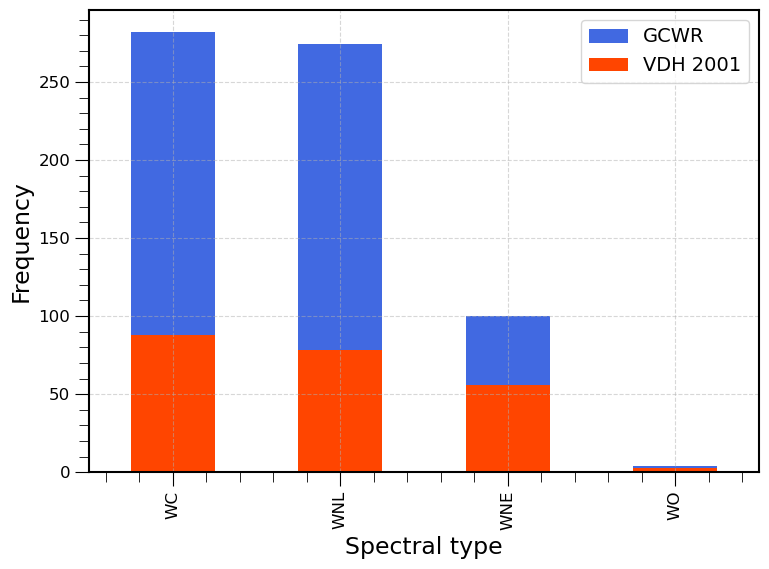
\includegraphics[width=0.7\textwidth]{chapters/introduction/image/spt_dist.png}
    \caption{Distribution of Galactic WR stars from \citetalias{van_der_hucht_viith_2001} and GWCR versus their spectral types.}
    \label{fig:dist_spt}
\end{figure}


\begin{figure}
    \centering
    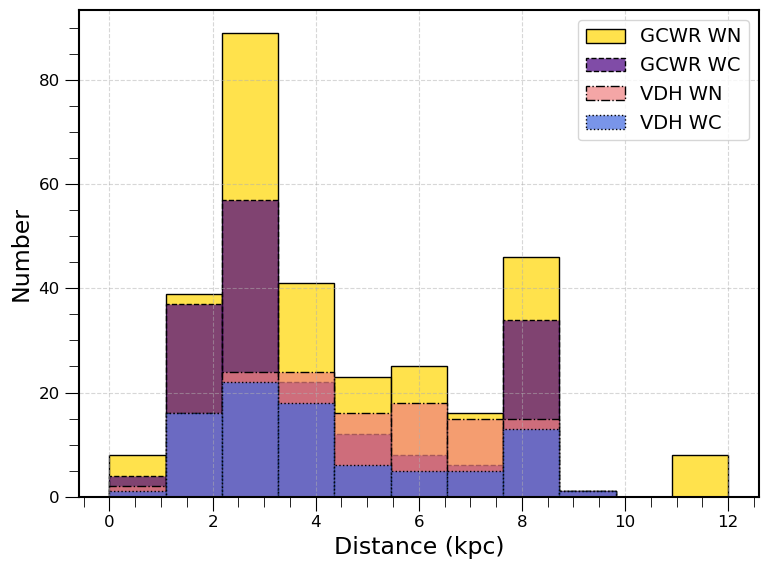
\includegraphics[width=0.7\textwidth]{chapters/introduction/image/dist_dist.png}
    \caption{Distances to Galactic WR stars from \citetalias{van_der_hucht_viith_2001} and GWCR.}
    \label{fig:dist_dist}
\end{figure}

% By nature of the initial mass function (IMF), classical WR stars are therefore mostly descendants of stars with initial masses in the range 25-75\,\Msun{}, and are usually hydrogen-free. However, there are a few classical WR stars that show lines of hydrogen in their spectra (e.g. WR 3). A large fraction of WNh stars are of spectral types WNL, and are main-sequence stars.

\subsection{Observed multiplicity properties}

% Numerous spectroscopic and imaging surveys have shown that the companion fraction of massive stars is high \citep[compilation by][]{2017moedistefano}. By investigating O stars in young, Galactic clusters, \citet{2012sana} computed that around half of O stars will interact with a companion over the course of their lifetime. This has drastic implications for the evolution of the star, while raising questions about the dominant evolutionary channel leading to the formation of WR stars.

When trying to understand the evolution of a binary system, it is important to define the orbital parameters: the period $P$, eccentricity $e$, inclination $i$, mass-ratio $q$, etc. Based on the evolution of the individual stars, these parameters will change over the course of their lifetimes. Knowledge of these parameters allows us to predict if binary systems interact, merge or become unstable. While there are more parameters to work with (as compared to single stars), binary systems offer the benefit of being able to measure the (minimum) masses of the individual components through Kepler's laws. This is extremely beneficial in the context of WR stars, since these direct measurements of dynamical mass and radius are valuable in constraining evolutionary models, of importance is the period distribution of the WR binary population, which help calibrate the physics of binary interaction in population syntheses codes.

The observed fraction of Galactic WR stars in binaries was reported to be ${\sim}0.4$ by  \citetalias{van_der_hucht_viith_2001}. This fraction is based on a compilation of 227 WR stars, of which 87 (43\% binaries) are of the WC sub-type, 127 WN stars (39\% binaries), 10 WN/WC stars. This includes very-long and extremely-long period binaries ($P>1000\,$d), and binaries identified through different methods (e.g. spectroscopy, visual binaries, photometry). Without going into details, we also examine the observed multiplicity at different metallicities. Through spectroscopic surveys, the multiplicity fraction of WR stars in the Large and Small Magellanic Clouds (LMC and SMC) were found to be ${\sim}0.3$ and ${\sim}0.4$ respectively \citep{bartzakos_magellanic_2001,foellmi_wolf-rayet_2003,foellmi_wolf-rayet_2003-1,schnurr_spectroscopic_2008}. At higher metallicities, \citet{neugent_close_2014} found that in the galaxies M31 and M33, the fraction of WR stars in short period binaries was ${\sim}0.3$. Although the number of WR stars in these galaxies are lower than those in our own and the detection of binarity probably more difficult, the observed binary fraction seems to be roughly independent of metallicity.


\begin{figure}
    \centering
    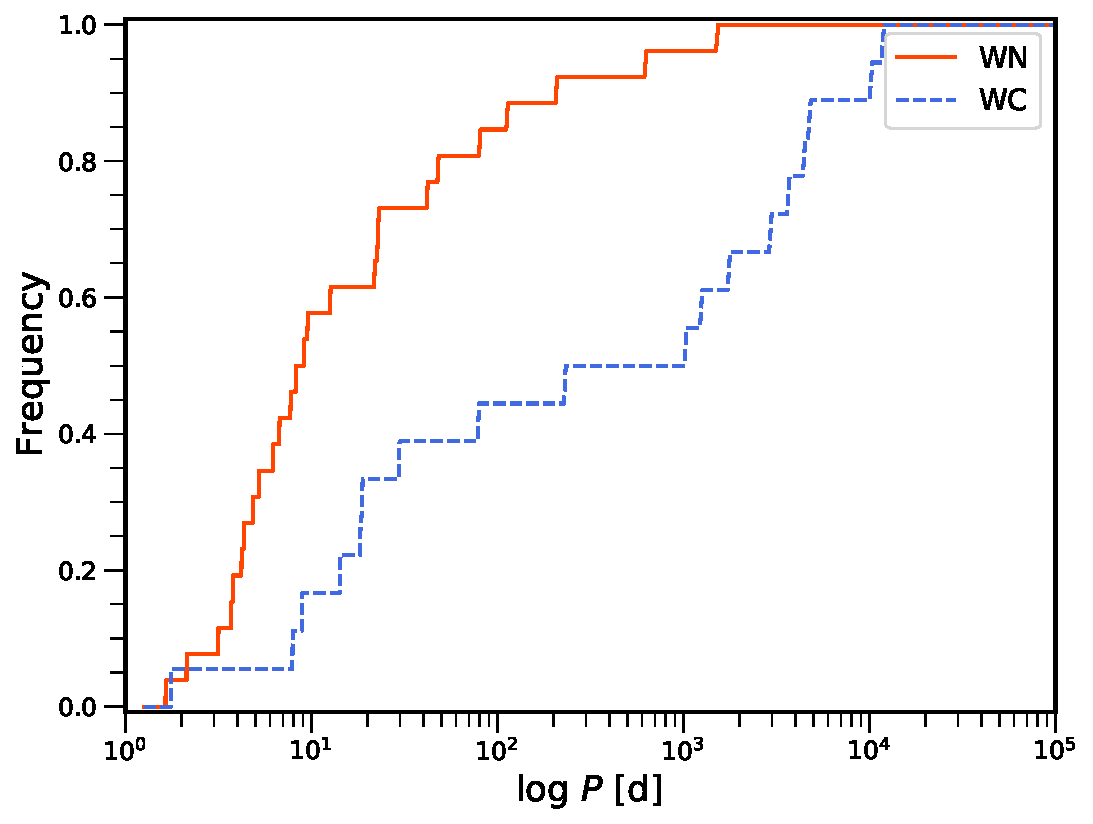
\includegraphics[width=0.7\textwidth]{chapters/introduction/image/Cumulative_pobs_withdust.pdf}
    \caption{Observed period distribution of Galactic WC and WN binaries from \citetalias{van_der_hucht_viith_2001}.}
    \label{fig:obs_pdist}
\end{figure}

Returning our attention to the Galactic population, the stars in the GCWR have not been examined for binarity in a homogeneous manner. The cumulative orbital period distribution from \citetalias{van_der_hucht_viith_2001} is presented in Fig. \ref{fig:obs_pdist}. It is clear that the period distribution of Galactic WC binaries is skewed towards longer periods compared to that of the WN population. While ${\sim}60$\% of WN binaries with known orbital periods have periods less than 10 days, the equivalent fraction for the WC binaries is only reached at orbital periods of ${\sim}$1000 days. An important distinction to highlight here is the lack, but not the absence, of short-period (10-100\,d) WC binaries when compared with the Galactic WN population. This is somewhat surprising, since short-period WR binaries should be the easiest to detect, given the large Doppler motion.

\textbf{Detecting Wolf-Rayet binaries}\label{sect:detection_methods}

Apart from orbital analysis, there are a multitude of techniques used to identify WR binaries. Depending on the orbital period, brightness-ratio, mass-ratio and inclination of these systems, different observational techniques allow for observers to detect WR binaries.

\textbf{Dilution of emission lines:} This technique only works when the brightness of the companion is comparable to the WR star. If a WR star is in a binary with an OB companion, the strength of the WR emission is theoretically diluted by the light from the companion \citep{1968aSmith,1989ContiMassey,2007Crowther}. However, if the companion is as bright or brighter than the WR star, then the composite spectrum of the system can even show absorption lines from the companion. Moreover, the strengths of emission lines of WR stars are not set in stone, and it is not always clear whether weak emission is the result of line dilution or weak winds.

\textbf{Identifying absorption lines in the spectrum:} This is a common technique used when it is difficult to obtain multi-epoch data on WR stars \citep[e.g.,][]{1989ContiMassey}. A high signal-to-noise, high resolution spectrum is often enough to detect absorption lines from a companion. However, some WR stars, especially at low metallicity \citep[e.g.,][]{hainich_wolf-rayet_2015}, show pseudo-absorption lines in their spectra, making them difficult to discern from a potential companion. Similar to the first method, this only works if the companion is comparable in brightness, even if the orbital period is of the order of years.

\textbf{Periodic change in the equivalent-width of spectral lines:} In WR stars that have strong line-profile variability, a technique to measure periodicity is through the equivalent widths of particular spectral lines. Such line-profile variability would occur if the companion was close enough for their winds to interact, i.e. with periods of a few days. However, the interpretation of this periodicity could also be co-rotating interaction regions, other large-scale structures in the wind, non-radial pulsations or an embedded neutron star/low-mass object in the wind of the WR star (see Sect. \ref{sect:wr_obs_char}).

\textbf{Spectroscopic monitoring campaigns:} Spectroscopic campaigns are another way of detecting WR binaries. As spectroscopy relies on detecting significant radial velocity (RV) variations in the WR star, it is highly sensitive to orbital periods up to a year, high inclinations and mass-ratios ($q=M_\textrm{WR}/M_2$) of the order of unity or higher \citep[see e.g.,][]{1998Marchenko1998WR141,2012David-Uraz,2021Richardson}. These systems can be classified as either SB1 (only one component detected in the spectra) or SB2 systems. The advantage of this method is that orbital solutions using Kepler's equations give us a model-independent method of determining minimum masses of the WR star and its companion. As mentioned before, this technique (and the previous two) are insensitive to small mass-ratios, as the companion would be too faint and too low-mass to induce RV variations in the WR star.

\textbf{Interferometric campaigns:} As the orbital period increases to more than a few years, spectroscopic campaigns are quite inefficient at catching these binaries. The increase in the orbital period also implies a larger physical separation, and this is where interferometry plays a significant role. At separations of 1-10 AU, long-baseline interferometry can resolve the visual orbits of WR binaries \citep[e.g. for WR 113 and WR 140, respectively:][]{2021Richardson,thomas_orbit_2021}. This translates to periods of 1 to ${\sim}20\,$yr.

\textbf{Infrared photometry:} Another technique used to monitor long-period WC binaries is through infrared photometry \citep{1995Williamsdust,1999MarchenkoDust,2001WilliamsDust,2005Williams,2019WilliamsNEOWISE}. WC stars are episodic dust makers, and the popular theory is that the WR\,+\,OB binary develops the right conditions to produce dust at periastron passage. These usually require decades of monitoring.

\textbf{Other techniques:} Lastly, long period binaries can be detected via imaging, X-rays from colliding winds or via non-thermal radio excess \citep[e.g.][]{1996Dougherty, 2000Dougherty, 2017Zhekov,2020Rodriguez, 2020Zhekov}.

\subsection{Correction for observational biases} \label{sect:obs_bias_intro}

The detection of binaries through spectroscopic campaigns mainly depends on the Doppler shifts of the WR line-profiles. These depend on the orbital parameters of the system, which we describe briefly. Any binary system can be defined by
% the following parameters:

\begin{itemize}
    \item orbital period ($P$) of the binary
    \item mass-ratio, defined here as ($q = M_{\textrm{WR}}/M_2$)
    \item eccentricity ($e$) of the orbit
    \item inclination ($i$) of the orbit with respect to the plane of the sky
    \item longitude of the ascending node of the secondary ($\Omega$)
    \item argument of the periastron of the secondary, measured with respect to the ascending node ($\omega$)
\end{itemize}

In a spectroscopic campaign, selected targets are observed with a particular combination of telescope/instrument for a certain amount of time. The total length of the observational campaign is called the \textit{time-base}, and the number of epochs observed spread out over the time-base is called the \textit{sampling}. The Doppler motion of the WR star is measured through RVs, which vary periodically over the orbital period. The semi-amplitude of the WR RV is called $K_{\textrm{WR}}$, and it is related to the orbital parameters listed above. The semi-amplitude of the secondary is called $K_2$. These amplitudes are directly related to the mass-ratio, through

\begin{equation}
    K_2/K_{\textrm{WR}} = q
\end{equation}

\begin{figure}
    \centering
    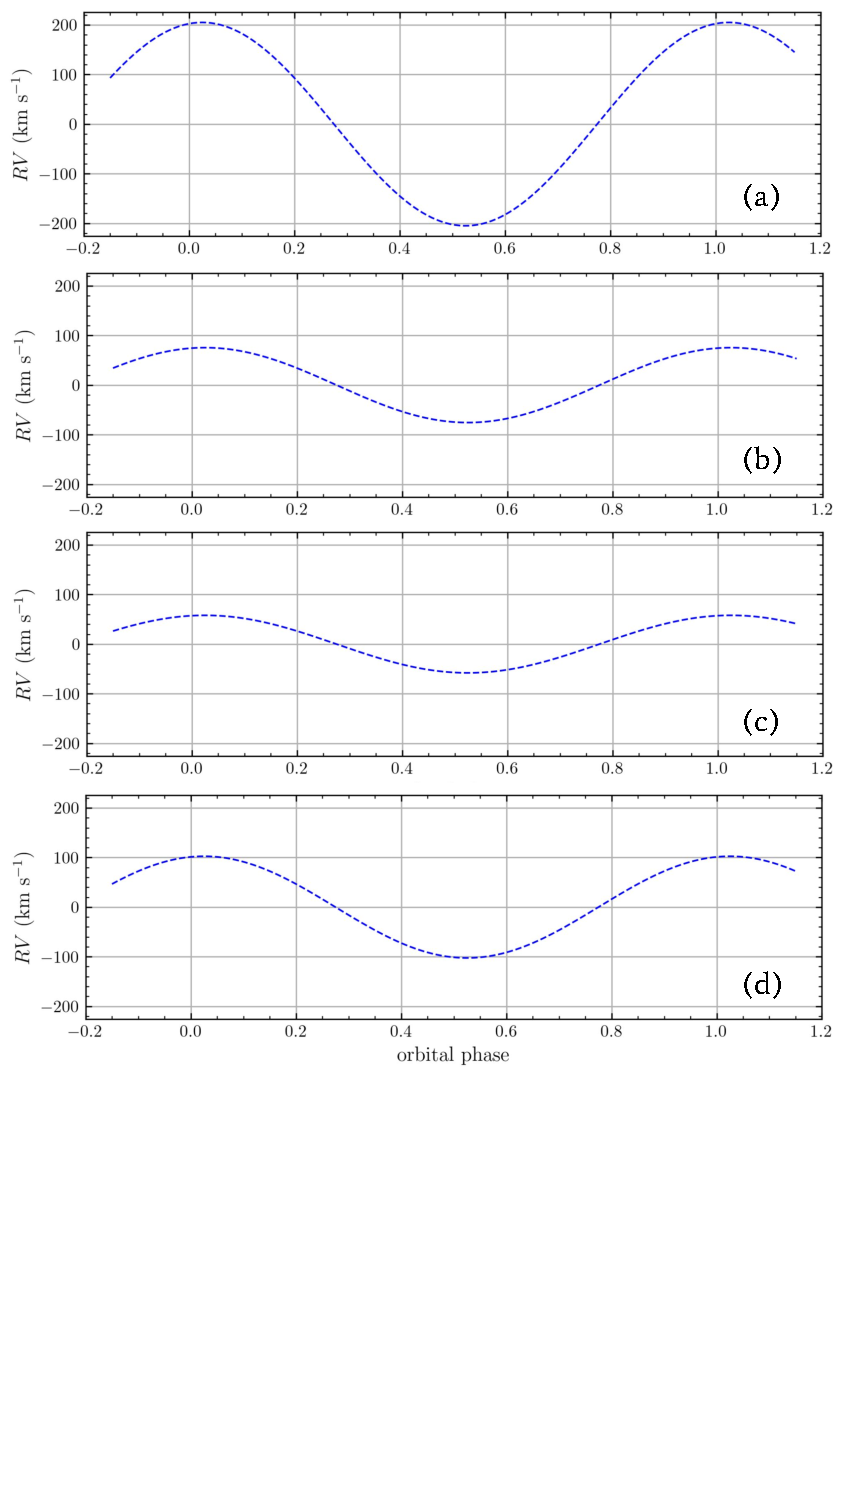
\includegraphics[width=\hsize]{chapters/introduction/image/Thesis_RV.pdf}
    \caption{Theoretical RV plots from spinOS \citep[][]{2021Fabry} for a star in a binary system with $P=15\,$d, $q=2$, $e=0$ and $i=90\degree$ (panel (a)). The change in \DelRV{} is shown by keeping all the parameters constant and varying (b) $P=300\,$d, (c) $q=0.33$ and (d) $i=30\degree$. }
    \label{fig:rv_model}
\end{figure}

As mentioned above, the orbital configuration of the system (or orbital phase, $\phi$) define the properties of the RV variations. As an example, we consider a binary system with $M_{\textrm{WR}} = 15\,$\Msun{} and $M_2 = 30\,$\Msun{}. For simplicity, the orbit is circular ($e=0$), implying the $\Omega$ and $\omega$ are not of consequence for now. With $P=15\,$d and $i=90\degree$, the theoretical RV curve computed with spinOS \citep{2021Fabry} can be seen in panel (a) of Fig. \ref{fig:rv_model}. By changing the period (panel (b), $P=300\,$d), mass-ratio (panel (c), $q=0.33$) and inclination (panel (d), $i=30\degree$) while keeping all other parameters constant, the RV variations, particularly the amplitude (\DelRV{}) change significantly. Clearly, the measured \DelRV{} is highly dependent on these parameters. To compound this problem further, the RV variation changes in an eccentric orbit and also depends on $\omega$ and $\Omega$. This implies that the time-base and sampling of the campaign have to be considered along with the aforementioned parameters when attempting to correct for observational biases.

Comparing panels (a) and (b) in Fig. \ref{fig:rv_model} shows that random sampling over a few epochs prefers the detection of shorter period systems as they exhibit larger RV amplitudes. Panel (c) shows a smaller \DelRV{} for the WR star with a low-mass companions. The effect of this bias can be seen in \citetalias{van_der_hucht_viith_2001} and the GCWR, as all of the currently known companions of Galactic WR stars are OB stars (except Cyg-X3, which is thought to be a black hole). This is understandable, because a WR star with a low-mass companion at a low inclination would be hard to detect, especially if the WR star has significant line-profile variability. Moreover, the detection of edge-on over face-on systems are preferred (Fig. \ref{fig:rv_model}, panel (a) versus (d)) as the Doppler shift in the line-of-sight is larger. Another potential bias that we discuss in Chapters \ref{ch:wne} and \ref{ch:wnl} is that of the sample selection relating to the brightness of WR stars. As mentioned before, a fair fraction of WR stars exhibit strong line-profile variability. This can significantly affect the RV measurements, which is why accounting for this while deriving the uncertainties on the RVs is crucial to account for this bias. Another uncertainty on the RV to account for is from the data-reduction and processing, along with the mathematical technique used to measure RVs. This is addressed in Chapter \ref{ch:wc}.

% Observational studies to determine the multiplicity have biases, depending on the method. For spectroscopy, the quantitative measurement that indicates if a star is part of a multiple system or not is the radial velocity (RV). If the star is in a binary system with parameters $P$, $i$, $e$ and $q$, then one would expect a velocity shift in spectral lines due to the Doppler effect based on the parameters of the system. Given a spectroscopic monitoring campaign of length, the measured RV amplitude (\DelRV{}) for this binary system depends on its parameters. In a spectroscopic campaign, it is not always known if the star is a binary, let alone these parameters. Therefore, the measured \DelRV{} suffers from a bias that must be corrected for. For example, if the eccentricity of the binary were $e=0.7$ and the observations were carried out when the binary was away from the time of periastron passage, then the RV amplitude measured would be small, and the system would then be classified as a single star.

% Apart from the systemic parameters, the observational bias also depends on the sample selection, instrument, data reduction techniques and analytic tools used. For an agglomeration of WR stars analysed with various techniques, correcting for the observational biases is not trivial whatsoever. Therefore, even though the observed multiplicity properties from \citetalias{van_der_hucht_viith_2001} are an extremely valuable first step towards understanding the binary population of Galactic WR stars, the intrinsic multiplicity properties are unfortunately out of reach.

\section{Motivation and outline of this thesis}\label{sect:motivation_intro}

There are numerous uncertainties that plague our understanding of massive-star evolution. Some of them include rotation, internal mixing, mass loss, binary interaction and magnetic fields. Handling all of this in a one-dimensional stellar evolution code only compounds the problem, as a deviation from spherical symmetry can be reached with more than one of the above parameters. As it is the post-main sequence phase of stellar evolution, the WR phase acts like a magnifying glass, highlighting the effects of these uncertainties. Studying the population of WR stars in a statistically significant manner provide an anchor point for stellar evolution models, using which we can work towards mitigating the shortcomings in our current knowledge. Additionally, WR stars are also progenitors of black holes, either via core-collapse SN or through direct collapse. The mass, multiplicity fraction and orbital configurations of WR stars directly give us insight on the future population of GW progenitors. Moreover, WR stars are suspected to be progenitors of GRBs, and the multiplicity properties of the WR population might help in understanding more about this phenomenon.

With this in mind, the following questions are of interest to us: what fraction of Galactic WR stars reside in binaries? What are the orbital configurations of these binaries? Do they give us insight into past events of binary interaction from the main-sequence phase (e.g. mergers, ejections)? Is the observed discrepancy in the orbital period distribution between WN and WC stars real, or is it simply a bias? What is the effect of multiplicity on the Conti scenario?

To attempt and constrain the intrinsic multiplicity properties of Galactic WR stars, we undertook a homogeneous spectroscopic monitoring campaign using the HERMES spectrograph mounted on the Mercator telescope on La Palma. From 2017-2021, we monitored 39 northern WR stars and obtained at least six epochs, and calculated the observed multiplicity fraction. We then corrected this fraction for observational biases and obtained the intrinsic multiplicity properties of the Galactic WR population.

In Chapter \ref{ch:data_reduction}, we introduce the instrument and data reduction techniques used in a homogeneous fashion. We developed an additional reduction scheme on top of the standard HERMES pipeline to correct for the instrumental response, and used continuum models to normalise the spectra.

In Chapter \ref{ch:wc}, we focus on the pilot study of 12 WC stars, where the methods in Chapter \ref{ch:data_reduction} were applied. We use cross-correlation to measure RVs, after which we identify the observed binary fraction. We then use Monte-Carlo simulations to quantify the detection probability in our sample across the relevant parameter space, and apply a correction for observational biases.

In Chapter \ref{ch:wne} we apply the above techniques to analyse a sample of 16 WNE stars. We develop a Bayesian framework around Monte-Carlo simulations, using which we calculated the power-law index, the upper and lower bounds of the period distribution along with the intrinsic multiplicity fraction of the WNE population. We re-visited the WC population and used these improved simulations to confirm what is observed in the literature, i.e. a lack of short period binaries. We compare what is obtained to main sequence O stars and discuss possible evolutionary consequences.

In Chapter \ref{ch:wnl} we round off our sample by analysing 11 WNL stars. We discover that the multiplicity properties are similar to those of the WNE population and run simulations for the combined WN population. After reconstructing the period distribution, we confirm that the addition of the WNL sample further strengthens our conclusions. We discuss possible binary evolutionary channels that could link the O, WN and WC populations and reproduce their multiplicity properties. Finally, Chapter \ref{ch:summary} summarises the work completed in this thesis and discusses future work.


%WR plus compact companion candidates have also been identified in external galaxies, IC 10 X–1 (Bauer & Brandt 2004) and NGC 300 X-1 (Carpano et al. 2007).



% In particular, massive stars with initial masses M$_i \gtrsim 8$\,\Msun{} are rare \citep{}, live short lives \citep{} and

% die with spectacular explosions called core-collapse supernovae \citep{}.

% Massive stars possess strong radiation-driven stellar winds \citep{cak1975} and are quite luminous, through which they affect the evolution of their host galaxies in numerous ways. They can trigger or inhibit star formation \citep{}, invest energy and angular momentum into the surrounding interstellar medium \citep{} and are the progenitors of neutron stars and black holes (BHs). They are also thought to be the progenitors for long-duration gamma-ray bursts (GRBs ??).

% Based on their initial mass, the Conti scenario has been slightly modified to reflect different evolutionary scenarios involving WR stars. For $M_i \gtrsim 75\,$\Msun{},

% \centerline{O $\xrightarrow{}$ WN (H-rich) $\xrightarrow{}$ LBV $\xrightarrow{}$ WN (H-poor) $\xrightarrow{}$ WC $\xrightarrow{}$ SN Ic,}

% whereas for ${\sim}40 \le M_i \le 75\,$ \Msun{},

% \centerline{O $\xrightarrow{}$ LBV $\xrightarrow{}$ WN (H-poor) $\xrightarrow{}$ WC $\xrightarrow{}$ SN Ic,}

% and for ${\sim}25 \le M_i \le 40\,$ \Msun{},

% \centerline{O $\xrightarrow{}$ LBV/RSG $\xrightarrow{}$ WN (H-poor) $\xrightarrow{}$ SN Ib.}

% By nature of the initial mass function (IMF), classical WR stars are therefore mostly descendants of stars with initial masses in the range 25-75\,\Msun{}, and are usually hydrogen-free. However, there are a few classical WR stars that show lines of hydrogen in their spectra (e.g. WR 3). A large fraction of WNh stars are of spectral types WNL, and are main-sequence stars.

% \begin{figure}
%     \centering
%     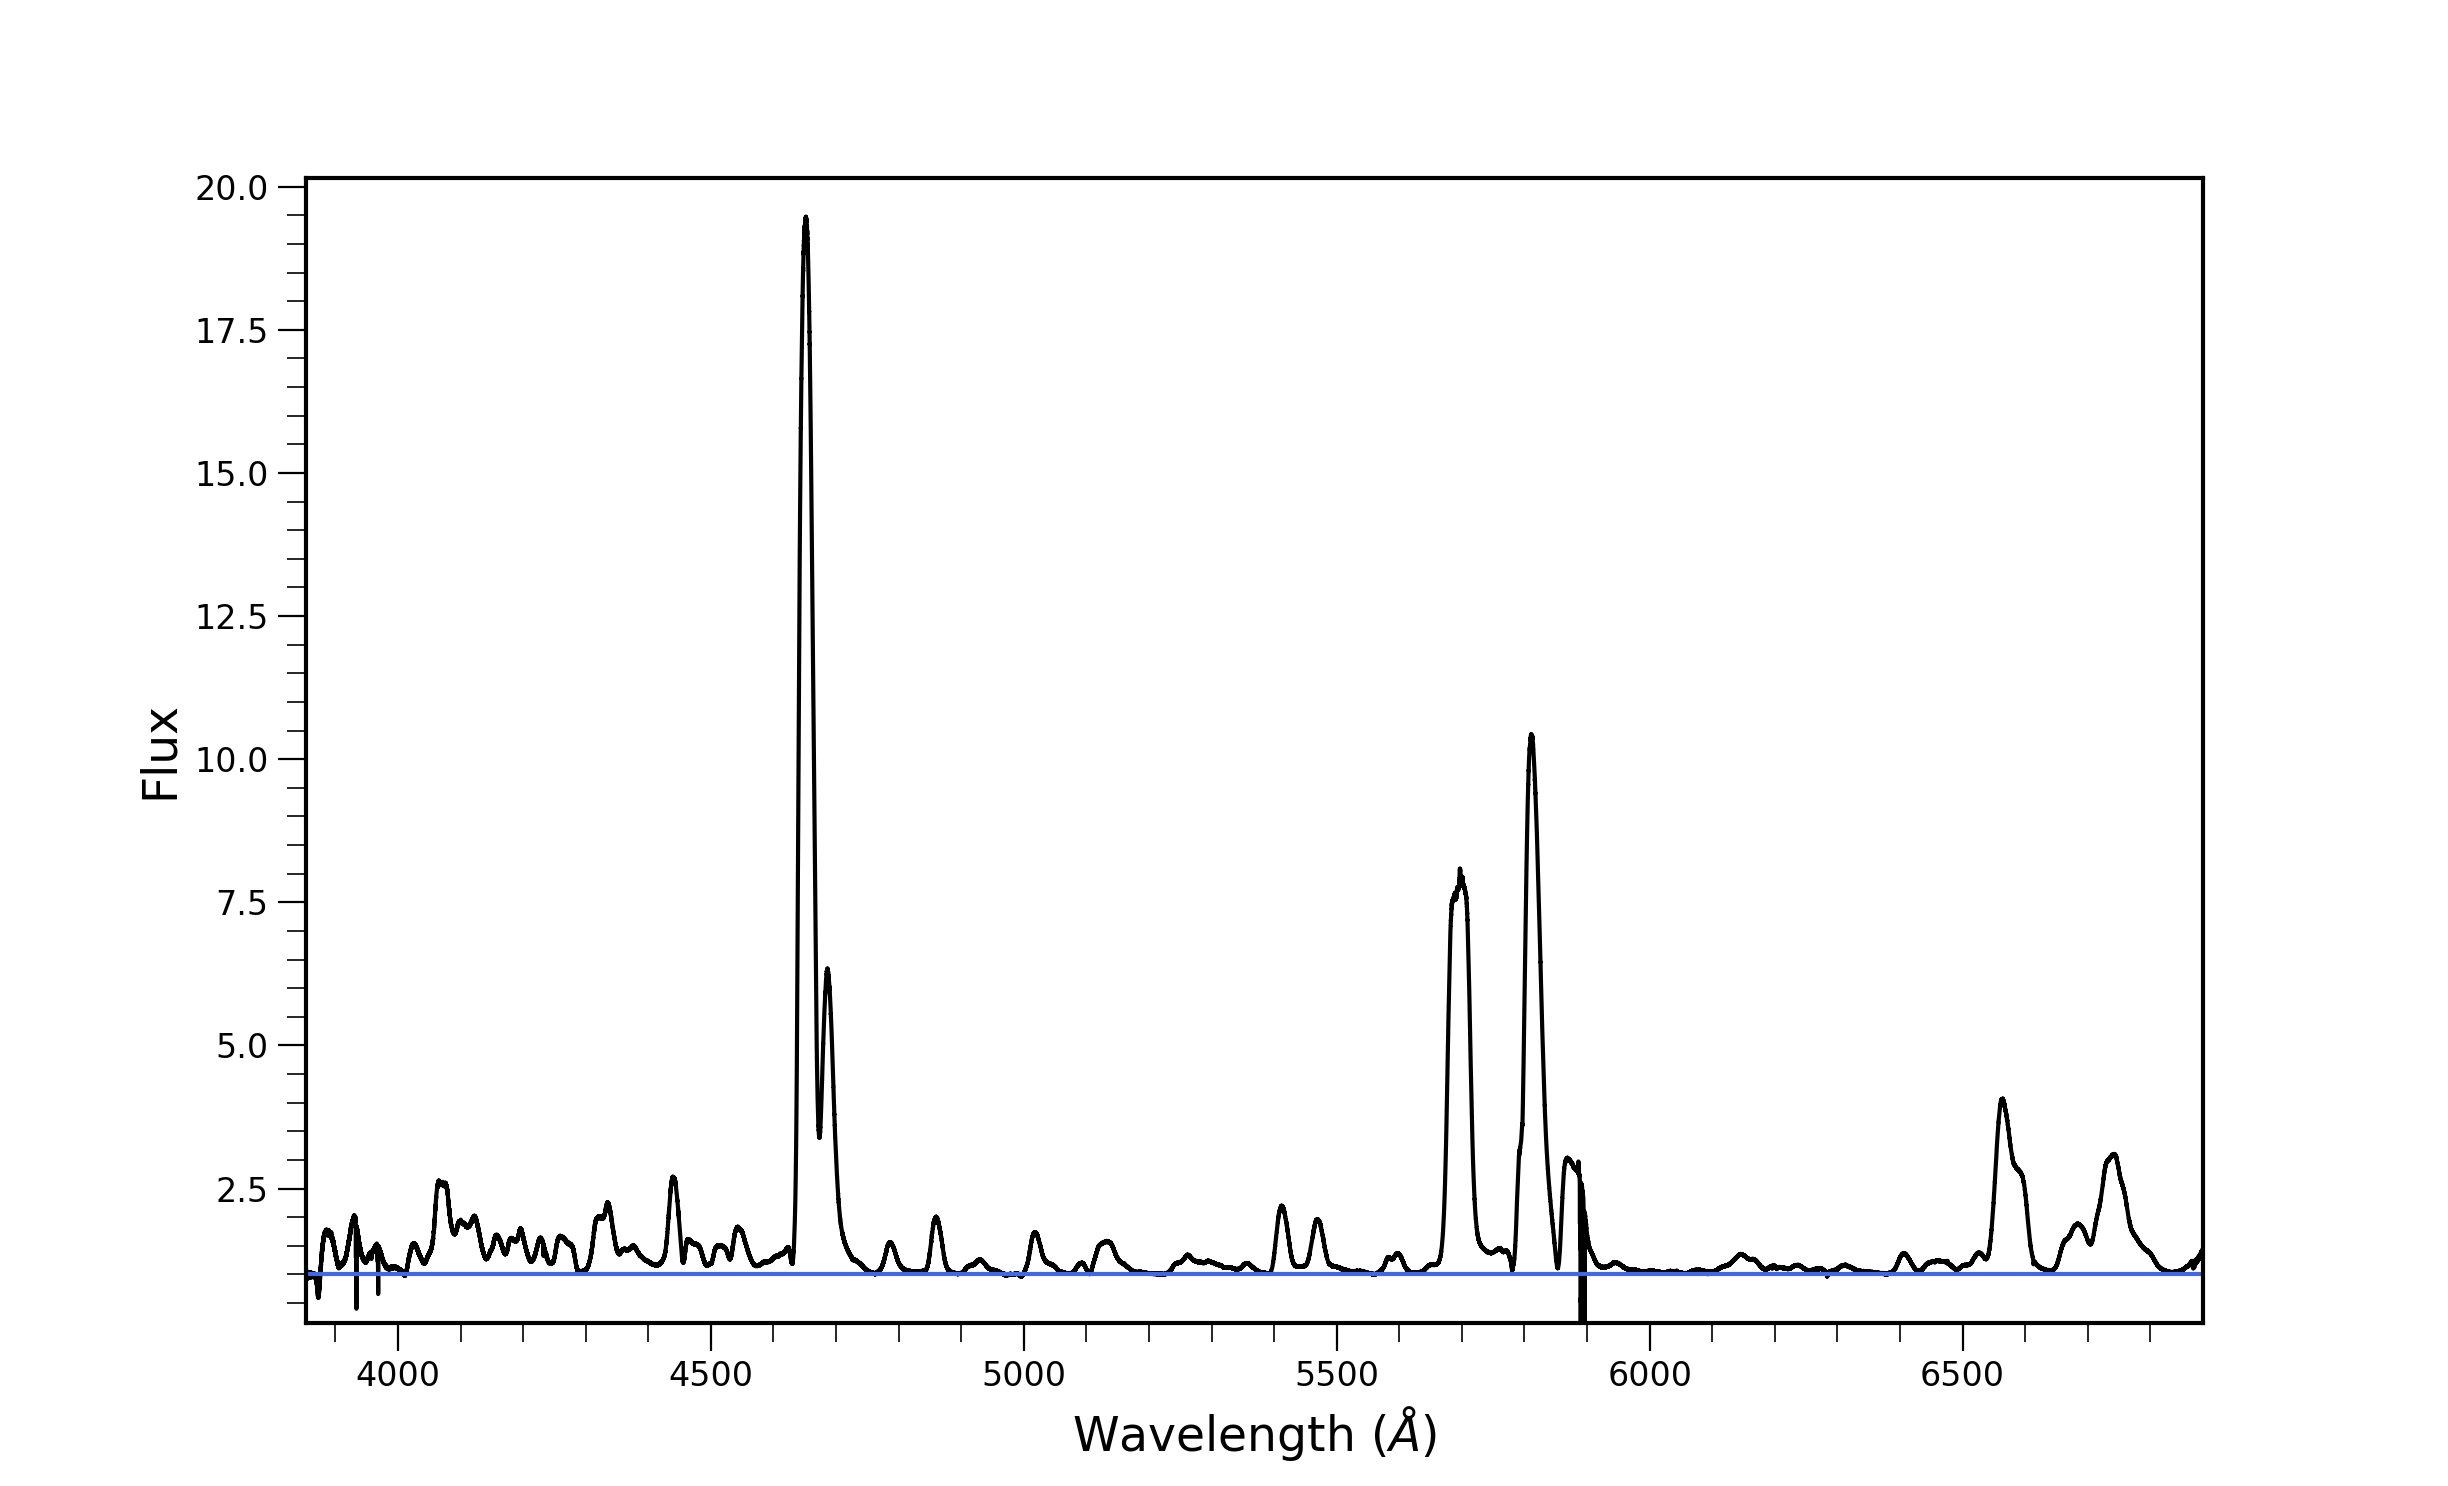
\includegraphics[width=\textwidth]{Chapters/introduction/image/WR135.png}
%     \caption{Optical spectrum of WR 135, one of the three Wolf-Rayet stars that were part of the initial discovery. The continuum level is indicated by the solid blue line.}
%     \label{fig:intro_wr135}
% \end{figure}




\cleardoublepage
